\section{Method}


\subsection{Cloud Infrastructure}
Public cloud being the most preferred choice for enterprise grade application deployments where the microservice communication and security 
is handed over to Istio, this research is conducted on \acrlong{gcp}. \acrshort{gcp} remains the choice as public cloud provider for this 
research project mainly because of the author's familiarity with the platform. As Istio works at Kubernetes environment level, all the 
methods used in this research are conducted on \acrlong{gke} - the fully managed Kubernetes service offered by \acrshort{gcp}.

\subsubsection{High Level Strategy}
To maintain a consistent and steady approach for each deployment and testing stages, \acrfull{iac} is used with Terraform. A rapid cloud infrastructure provisioning and de-provisioning model is followed to keep the cloud cost minimal. All the Terraform IaC, Shell scripts and Kubernetes configurations files used in this research are available at \ref{appendix:researchRepo}. At a high level first the Kubernetes cluster is provisioned and verified by kubectl on local system. Next the observability stack is installed on the cluster followed by the service mesh itself is installed and verified. After all the platform level stuffs are installed, configured and verified, a demo web application \acrfull{boa} is deployed using Kubernetes manifest files including the front end microservice attachment to the Istio ingress controller. This enables the application to be accessed from outside of the cluster. At the end of each testing sessions, everything is teared down completely using \acrshort{iac} to save cloud cost.

\subsubsection{Terraform Provisioning}
\acrfull{iac} used in this research leverages several Terraform modules to provision the \acrshort{gke} cluster along with necessary cloud components like \acrshort{vpc} network, subnet and node pool. Google offers several Terraform APIs to customize the cluster resource provisioning which gives a greater control and easy management of \acrshort{gke} cluster. For an easy identification of cluster resources, custom IP ranges are defined in Terraform script for Kubernetes services and pods. As a prerequisite of this setup a GCP project and service account is created manually from \acrshort{gcp} console along with enabling all required APIs using gcloud command line tool on local system. Terraform script defines the following configurations for the cluster used in this research. 
\begin{itemize}
    \item europe-west1 region 
    \item e2-standard-2 machine type
    \item 1 minimum cluster node
    \item 10 maximum cluster nodes
    \item 2 initial nodes
\end{itemize}

Essentially, a zonal cluster is created in europe-west1 region located physically at Belgium (\cite{gcpDocRegion}). This features a custom node pool started with 2 nodes and scaled up to 10 nodes. The machine type for the nodes are e2-standard-2 offering 2 vCPU and 8GiB RAM. Kubernetes version is set to v1.27.3 which is one of the most recent and stable release of Kubernetes (\cite{kubeDocRelease}) at the time of writing this paper.


\subsubsection{Demo Application}
\acrshort{boa}, a microservice based demo application from \acrshort{gcp} open source repository \cite{githubBOA} is used for this research project. This application is developed by \acrshort{gcp} team to demonstrate their products and proven to be a perfect fit for evaluating Ambient mesh as it comes with predefined Kubernetes deployment manifest files. With minimal changes to these manifest files, microservice deployment remains fairly straight forward job for the research. This enables focusing more on the Istio rather investing more time on application source code build and deployment. \acrshort{boa} simulates a virtual online banking system with facilities of account opening, deposit, withdraw and balance enquiry. This application consists of a total nine microservices out of which, eight microservices are used without any modifications for this research. The application follows a typical microservice based architecture which is defined in Figure \ref{method:boaDesign}.

\begin{figure}[ht!]
    \centering
    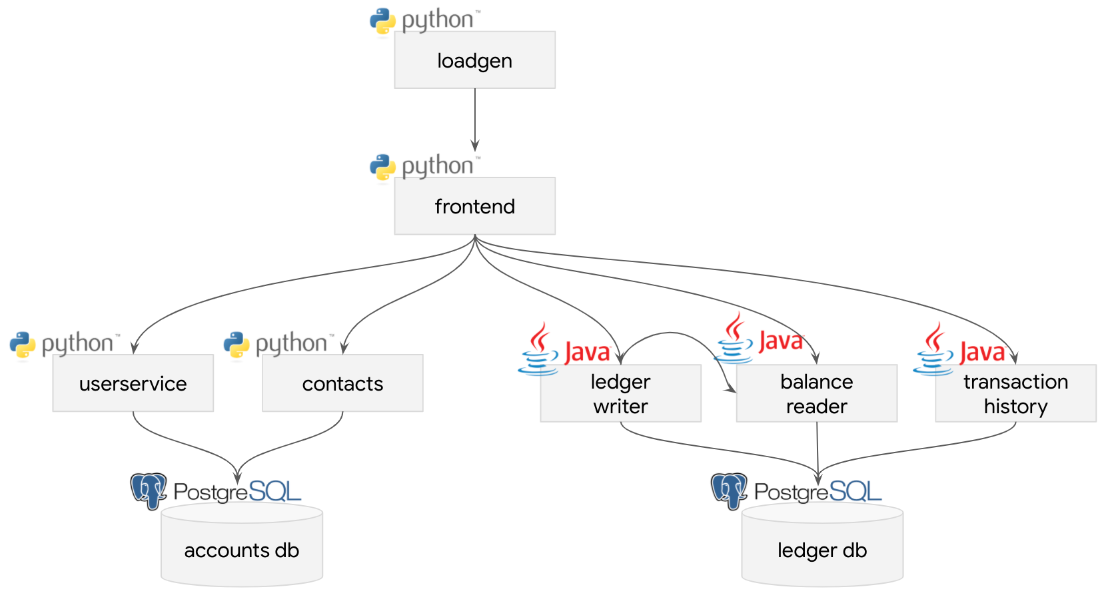
\includegraphics[width=1.0\linewidth]{resources/boa-architecture.png}
    \caption{Bank of Anthos application architecture}
    \label{method:boaDesign}
\end{figure}

The load generator script comes with the project is modified to suite the purpose of this research and run from local system to reduce the burden on the cluster.


\subsection{Observability System}
Monitoring in dynamic service-oriented architectures is a crucial point of success and observability takes it all to a complete new level by exploring the internal state of the microservices. This paper explores the resource utilization of ambient mesh in different conditions and compares them with Istio's sidecar models utilization. To perform this comparison, collecting time series data points, storing and visualizing them is very crucial, hence a rich observability stack named Prometheus and Grafana is used.

\subsubsection{Prometheus as Datasource}
To describe what Prometheus is, a quick introduction to metrics is required. Metrics are numerical measurements based on which a decision or an internal state of an application can be assessed at a particular point in time. Prometheus collects and stores these metrics in a time series database for further analysis by other tools. In a nutshell Prometheus is an open-source system monitoring and alerting toolkit which uses time series database. It offers a robust data model and a query language called PromQL which will be leveraged in Grafana dashboard for the purpose of this research.

\subsubsection{Grafana as Visualizer}
While Prometheus remains pioneer at collecting and gathering metrics from microservices for a prolong time, visual representation and report generation cannot be made easier in anything than Grafana. Grafana works as an aggregator for all data sources and exploring data to pinpoint the required thing in log, metrics or traces. The biggest advantage of using Grafana over native Prometheus for visualization is the rich UI elements that it offers. So, in this research for ease of research result understanding and prominent data points, Grafana will be used.

\subsubsection{Prometheus and Grafana Setup}
Prometheus community helm chart is used to install the observability stack which comes by default with Prometheus, Grafana, Node exporter and Alert manager. A dedicated namespace 'monitor-system' is used for all these Kubernetes deployments and verified using k9s - a tool to interact with Kubernetes cluster. With this installation in place, Prometheus agent starts metric collection from all Kubernetes pods and sent to Grafana instance. For rest of the research, the Grafana deployment is used with Kubernetes port forward feature on local system to access the monitoring dashboard. A custom dashboard (\cite{soloGithubPerf}) is imported in the live instance of Grafana to capture the research test results. A minor customization (Appendix \ref{appendix:researchRepo}) is done on top of the imported Grafana dashboard to enhance the graph visualization and having the required namespace filters in place.


\subsection{Test Architecture}
Ambient mesh does not rely on any additional containers in microservice pods, the memory and CPU footprints shall be lower on the overall system, including pod, node and cluster levels. In sidecar mode, Istio deploys a sidecar proxy per pod, and this sidecar increases proportionally with the pod replica counts. Ambient mode deploys Ztunnel proxy per node and Waypoint proxy per service account or namespace basis. Istio system load comparison across multiple microservice pods and cluster nodes shall account for these factors while testing. Istio shall be used with default mTLS inter-service communication and an L7 policy in ambient mode to engage the Waypoint proxy. Overall, the two deployment scenarios with the BOA application shall deliver a result on the performance factor of ambient mesh. Data collection shall be performed on the site data plane across the cluster using Prometheus and Grafana.

\subsubsection{Compute Resource Utilization}
First, a typical use case of small organization shall be followed where 8 microservices of the BOA application is deployed to a single Kubernetes namespace with two replica counts. Secondly, an enterprise grade deployment model shall be followed where microservices are typically deployed in different namespaces with team level access restriction applied by Kubernetes role based access control (RBAC) policies. The RBAC is not applicable here as that has no impact on service mesh performance but BOA microservices shall be deployed to 8 different namespaces with 6 replicas. This test will verify the Waypoint proxy performance impact in an enterprise grade environment as 8 Waypoint proxies will be in the cluster attached to each namespaces. In both cases, the count of Ztunnel proxies will vary based on the cluster node count. The exact test config data shall be captured in test result section including the test data comparison between the sidecar mode, ambient with L4 proxy only and ambient with L4 and L7 proxies. A load testing tool comes with BOA application shall be used to simulate traffic data to BOA for 10 minutes in each cases with 50 users at a rate of 1 per second to perform sign up, login, transaction and logout operations. Two architectures are depicted below about the test infrastructures.

\begin{figure}[ht!]
    \centering
    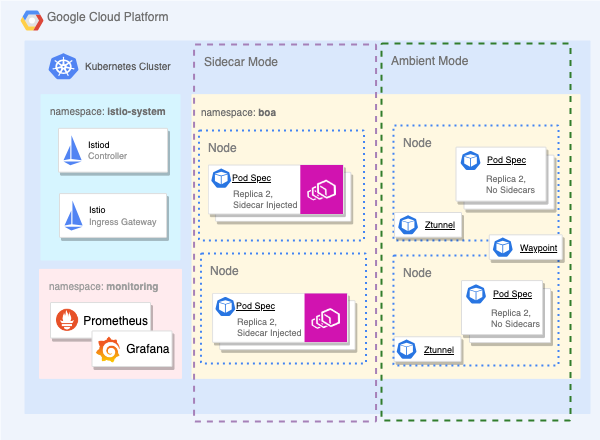
\includegraphics[width=0.7\linewidth]{resources/single-ns-test-infra.drawio.png}
    \caption{GCP infrastructure architecture with single namespace for test}
    \label{method:singleNsInfraArch}
\end{figure}

\begin{figure}[ht!]
    \centering
    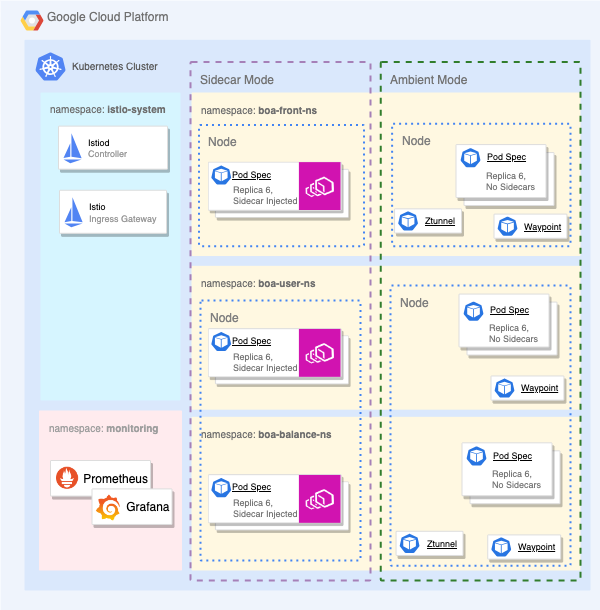
\includegraphics[width=0.7\linewidth]{resources/multi-ns-test-infra.drawio.png}
    \caption{GCP infrastructure architecture with Multiple namespace (diagram shows only 3, actual test uses 8) for test}
    \label{method:multiNsInfraArch}
\end{figure}

\subsubsection{Latency Impact Measurement}
Grey literature mentions Istio’s network latency and identifies the source as intensive L7 processing (\cite{istioHoward2022}). In ambient mesh, the L7 or Waypoint proxies can be deployed to different nodes by the Istio system. This situation directs the Ztunnel to pass traffic through a Waypoint deployed on a separate node, adding some delay in microservice calls. Istio authors claim the latency is close to Istio sidecar implementation (\cite{istioHoward2022}). A test comparison between the sidecar and ambient mode of Istio shall reveal the result of this claim by measuring latency between two microservices from the BOA application. This latency test will also decide whether separating proxy layers among L4 and L7 in ambient mode results in some practical benefits.

\subsubsection{Operational Complexity Measurement}
On a live Kubernetes cluster with hundreds or thousands of microservices, upgrading Istio is always a challenge for Kubernetes admins. To minimize the impact, Istio documentation (\cite{istioDocCanaryUpgrade}) recommends to use blue-green deployment and canary deployment strategies to roll out new versions of Istiod control plane and ingress controller respectively. Upgrading Istio using these strategies are highly dependent on Istio Canary Deployment feature (\cite{istioDocHelm}) which is fortunately available in both the Istio versions used in the test. Aim for this test remains at comparing the sidecar and ambient mode from a service downtime and upgrade complexity perspectives. As recommended by Istio community, a blue-green deployment strategy is used to upgrade Istiod whereas canary deployment is used for ingress controller upgrade. Grafana is used to capture service downtime monitoring during Istio upgrade process by tracking HTTP response code 200. Istio version 1.20.0 being the latest release (\cite{istioNewsVersion}) of Istio as of writing this research paper this test will be a state-of-the-art comparison report on Istio version upgrade as well. The Istio upgrade process will follow the architecture shown in Figure \ref{method:istioUpgradeArch}.

\begin{figure}[ht!]
    \centering
    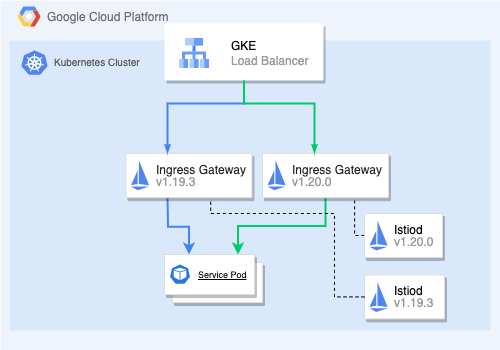
\includegraphics[width=0.7\linewidth]{resources/istio-upgrade-strategy.drawio.png}
    \caption{GCP infrastructure architecture while upgrading Istio to avoid downtime}
    \label{method:istioUpgradeArch}
\end{figure}

As the sidecar mode of Istio needs proxy injection during pod initialization phase, installing Istio in Kubernetes cluster after an application deployment remains a challenge for the operators. Fortunately most of the times this is not a concern as in enterprise level organizations, applications are deployed only after Kubernetes cluster is configured and validated with required elements including Istio. For academic purposes, this research will verify whether the Istio ambient mode offers a smooth transition from no mesh to service mesh when Istio is installed post application deployment on a Kubernetes cluster.


\subsection{Test Readiness}
As the open source edition of ambient mesh is now a part of Istio project, this research is focused on two modes of Istio - sidecar and ambient. Istio remains the core part of this research and to produce the research report on ambient mesh this paper explores the performance and operational complexity of Istio ambient mode. A deep dive is made in this section on how Istio is installed, configured and verified in two different modes. Istio documentation (\cite{istioDocInstall}) refers Istioctl tool to be the preferred installation method for Istio being the most well managed and secured path. However for the Istio upgrade test the helm chart method is used in this research. Under the hood Istioctl method uses helm chart to install and configure Istio but using Istioctl tool comes with some additional benefits like quickly deploy an ingress gateway or monitoring tool instances for test purposes. Two most recent releases of Istio are used in this research - v1.19.3 and v1.20.0. To install Istio, Istioctl is downloaded to local system where the cluster communication is already established from previous steps. A clean installation of Istio with Istioctl brings up 2 core components of Istio, Istiod - the control plane and the ingress controller. These remains valid for both sidecar and ambient modes without any differences.

\begin{figure}[ht!]
    \centering
    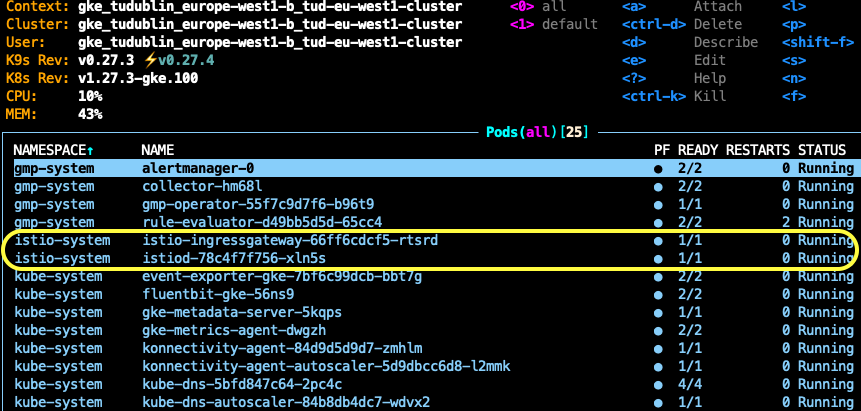
\includegraphics[width=1.0\linewidth]{resources/istio-std-installed.png}
    \caption{Istio sidecar deployment}
    \label{method:istioStdInstalledView}
\end{figure}

As part of the installation, a namespace istio-system is created where both the components are placed. The ingress gateway will serve the frontend microservice over public IP address whereas the Istiod will configure all the sidecar proxies in application namespaces. Istioctl creates a istio-system namespace by default for all the Istio system services and pods.


\subsubsection{Sidecar Mode}
At this stage application namespace labelling is done with 'istio-injection=enabled' to configure Istio system for sidecar injection into application pods. On the application deployment side, first the JSON web token is deployed to 'boa' namespace as a Configmap. Next, all the microservice manifests are deployed to set up the application workload and services. Once all the deployments are successful, the k9s view shows all microservice pods with two replicas each. Only the accounts-db and ledger-db microservices are deployed as a single StatefulSet. On checking the pod description using k9s, 'istio-proxy' container is seen representing the Istio data plane.

\begin{figure}[ht!]
    \centering
    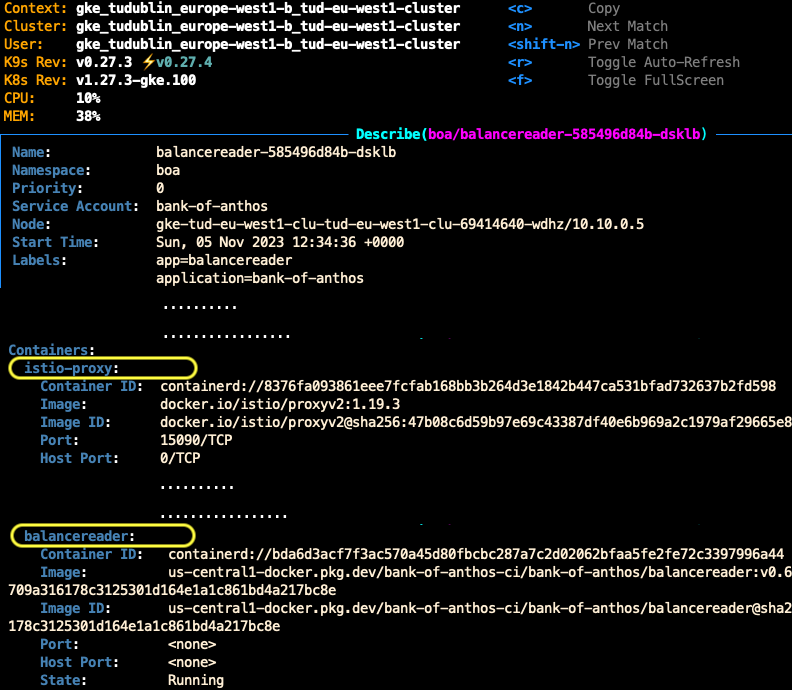
\includegraphics[width=1.0\linewidth]{resources/istio-sidecar-injection.png}
    \caption{Istio sidecar injection is in action}
    \label{method:istioSidecarInjectionView}
\end{figure}

After the above verification, the frontend gateway is deployed so that the application can be accessed from outside of the cluster and further tests can be performed. At this point, a verification is done whether Istio data plane is engaged to offer the basic service mesh features like mTLS communication between microservices. A sniffing plugin for kubectl is used on local system along with packet capturing tool Wireshark. First, the test is executed without Istio deployed to proof that HTTP communications between microservices happens over plain text followed by Istio's mTLS encryption. While comparing the packet sniffing results between frontend and balance reader microservice a balance value of 71580 is spotted in plain text as shown in \ref{method:plainTxtWiresharkView} when Istio is not deployed.

\begin{figure}[ht!]
    \centering
    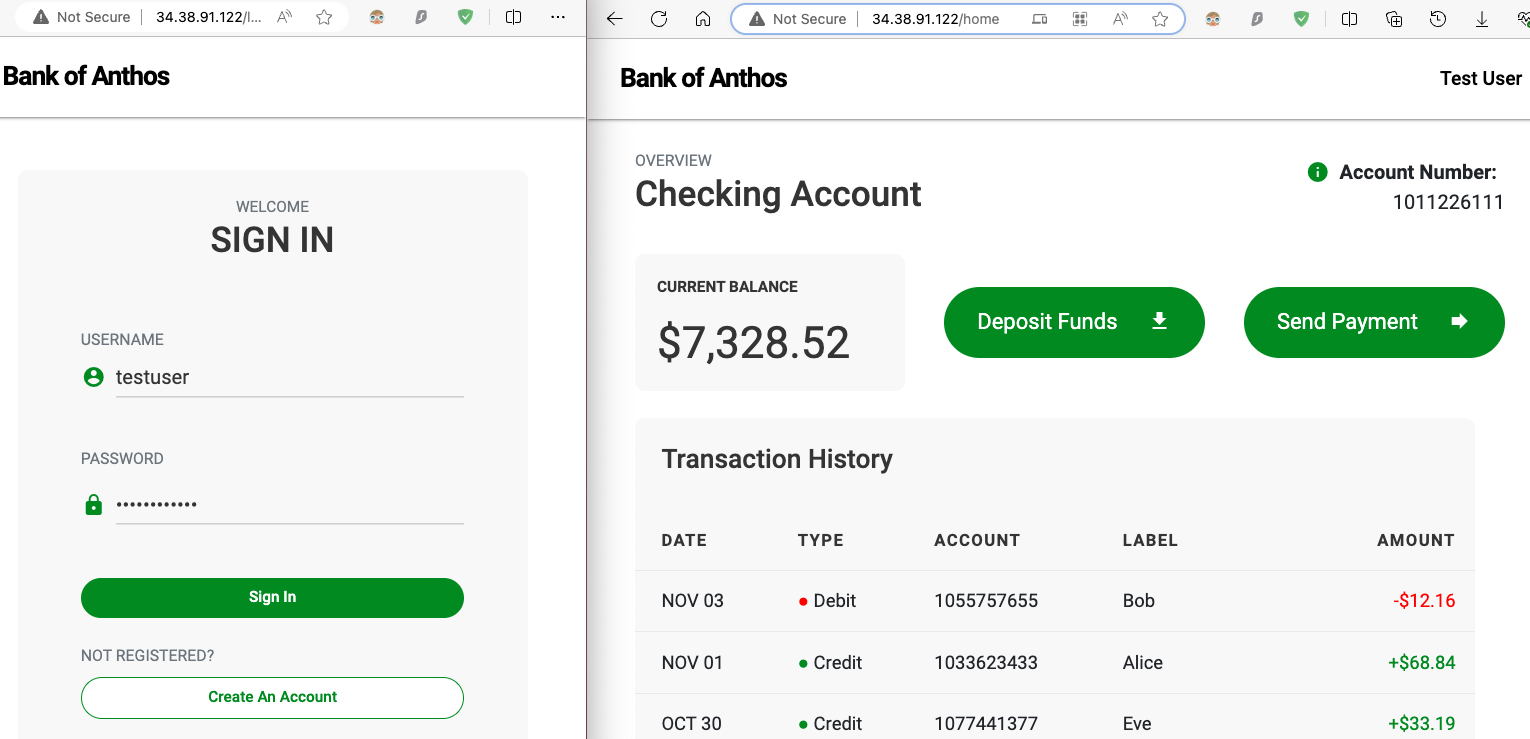
\includegraphics[width=1.0\linewidth]{resources/boa-view.png}
    \caption{Bank-of-anthos is accessible over external load balancer}
    \label{method:boaWebView}
\end{figure}

\begin{figure}[ht!]
    \centering
    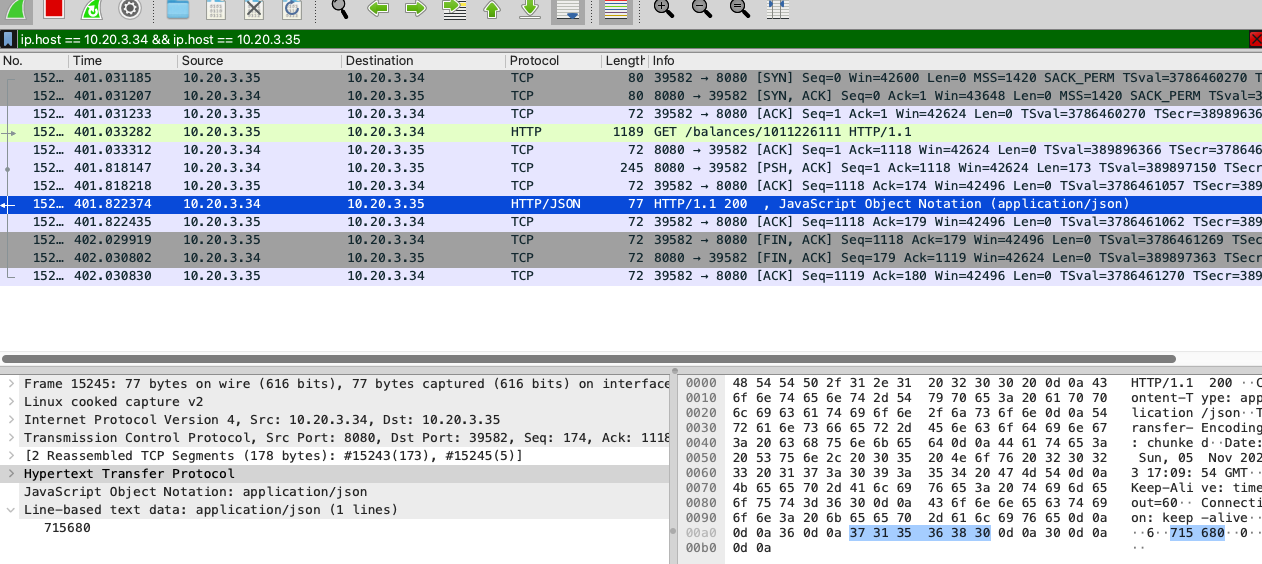
\includegraphics[width=1.0\linewidth]{resources/raw-balance-value.png}
    \caption{Plain text communication without Istio deployment captured in Wireshark}
    \label{method:plainTxtWiresharkView}
\end{figure}

\subsubsection{Ambient Mode}
Executing Istioctl install with ambient profile is used to set up the istiod control plane, Kubernetes CNI plugin and the Ztunnel proxy at host level. To deploy an ingress gateway, either couple of parameters needs to be passed to Istioctl command line or a config YAML need to be applied manually. Microservice deployment steps shall remain same but the application namespace label shall be changed to "istio.io/dataplane-mode=ambient" to engage ambient mode data plane. At this point, only Ztunnel component of ambient mesh is set up which can be tested by sending some traffic to pods and sniffing both pod and Ztunnel network to learn that, external traffic is only coming to Ztunnel pod. The following two figures shows how the Ztunnel is intercepting traffic received from ingress gateway 10.20.0.22 and then passing it through service pods.

\begin{figure}[ht!]
    \centering
    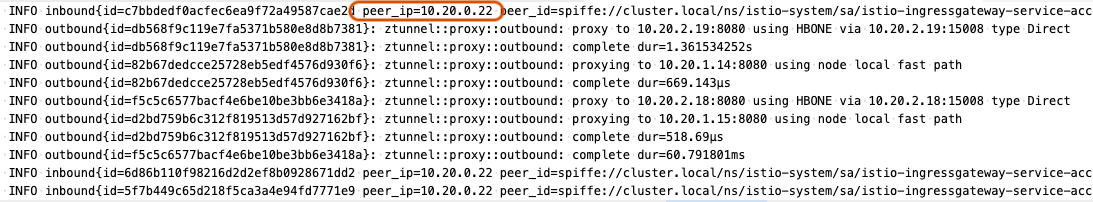
\includegraphics[width=1.0\linewidth]{resources/ztunnel-log.png}
    \caption{kubectl log view from Ztunnel pod}
    \label{method:ztunnelLogView}
\end{figure}

\begin{figure}[ht!]
    \centering
    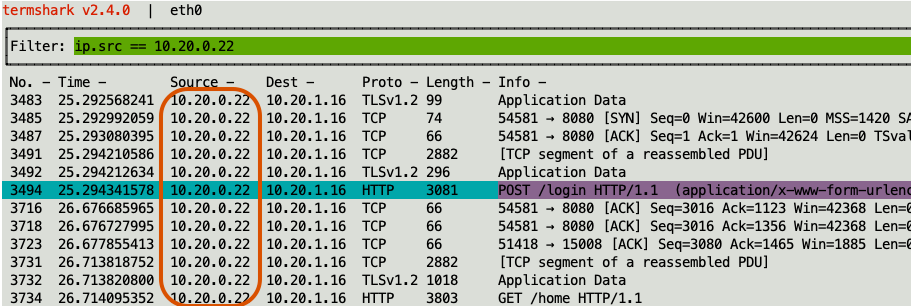
\includegraphics[width=1.0\linewidth]{resources/ztunnel-network-trace.png}
    \caption{Ztunnel network traffic captured from TermShark}
    \label{method:ztunnelTraceView}
\end{figure}

The Waypoint proxy set up need Kubernetes gateway API CRDs as prerequisites. By default Waypoint proxy get installed per namespace wise. Hence this research will focus on couple of different configurations for Waypoint proxy - all microservices deployed in a single namespace mapped to a single Waypoint proxy and microservices deployed across multiple namespaces mapped to different Waypoint proxies. In grey literature, there is a few test results discussed among Istio's sidecar and ambient mode, but a comparison between Waypoint proxies deployed in single and multiple namespaces is not performed. Figure \ref{method:waypointAppliedView} shows how the Waypoint proxy is engaged in ambient mesh setup to the microservice pods.

\begin{figure}[ht!]
    \centering
    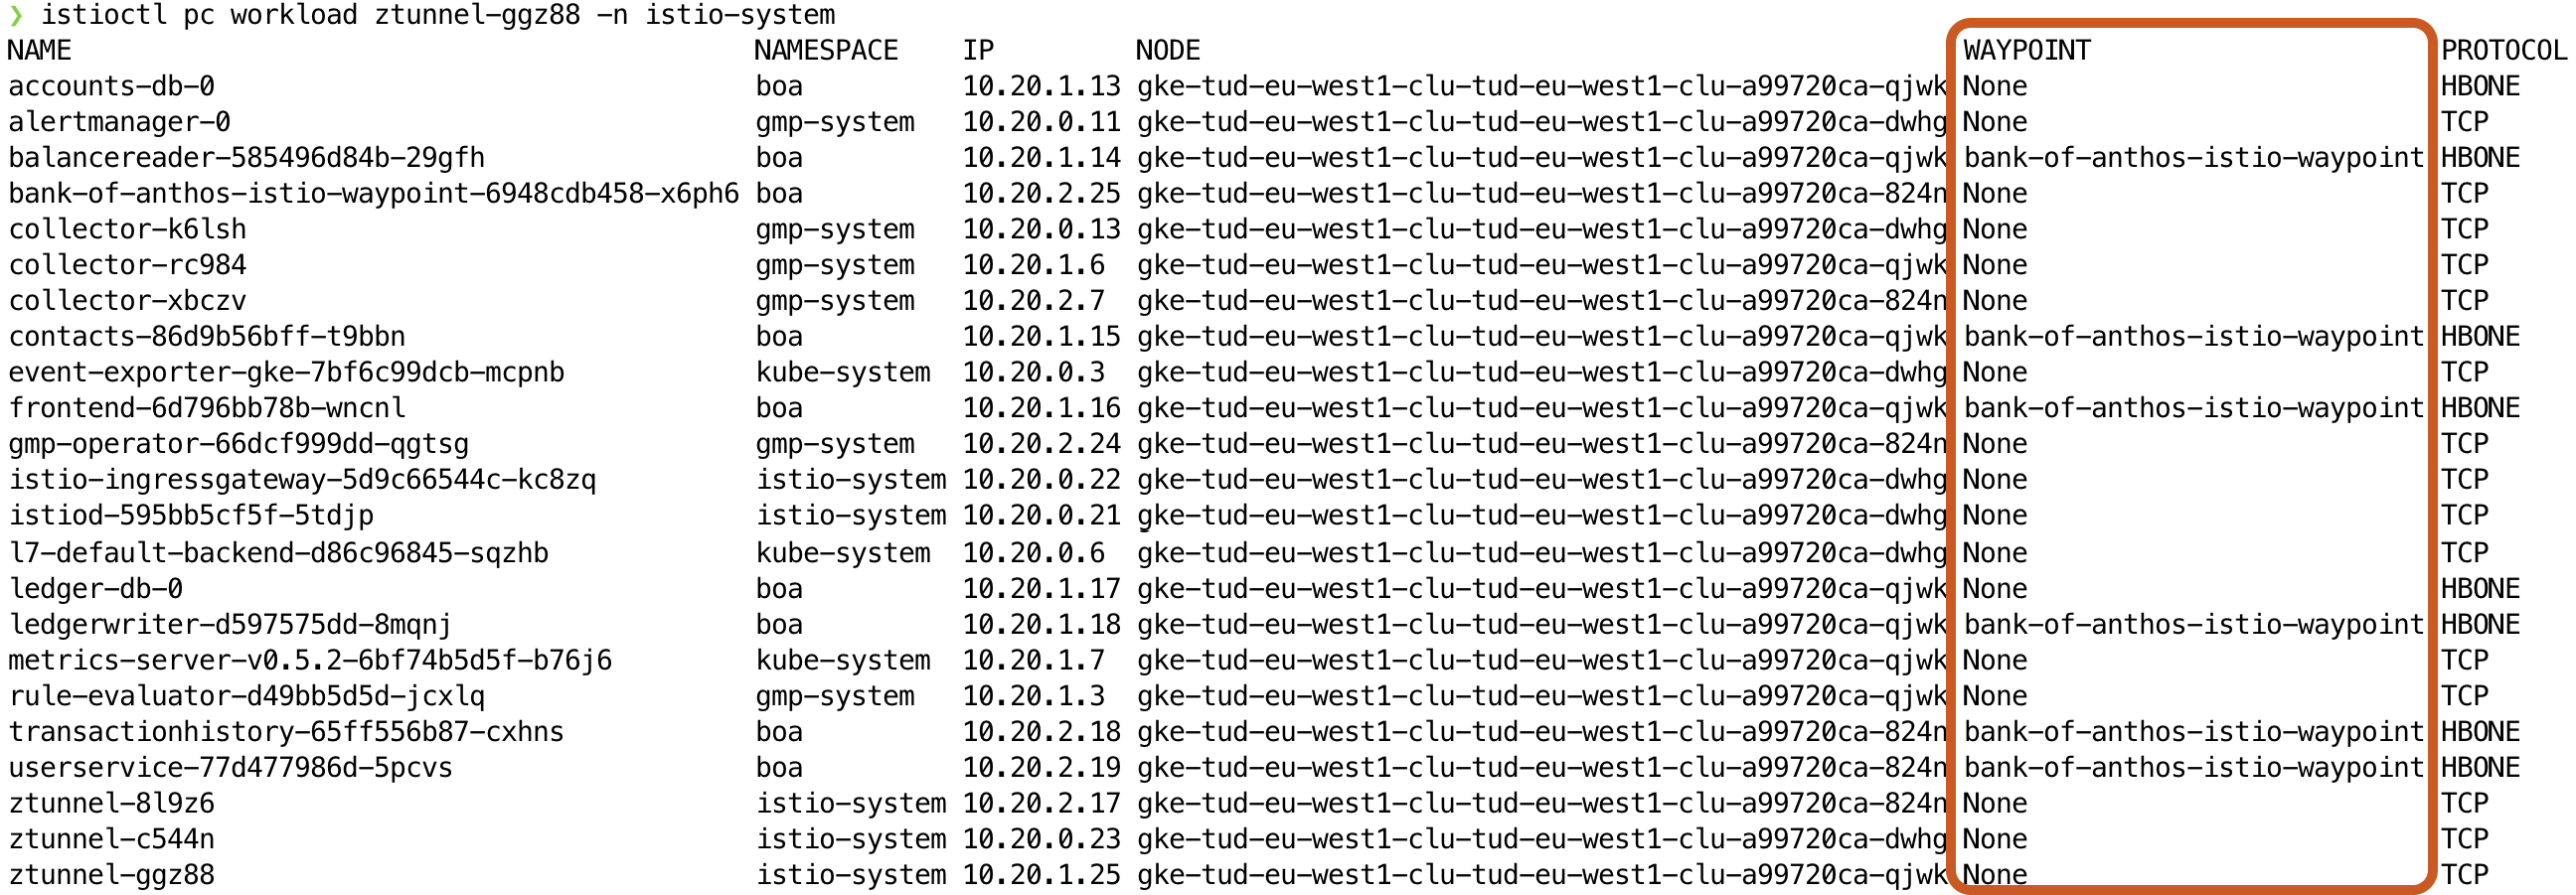
\includegraphics[width=1.0\linewidth]{resources/waypoint-applied.png}
    \caption{Waypoint proxy applied in ambient mesh}
    \label{method:waypointAppliedView}
\end{figure}

To see Waypoint proxy engagement, a L7 policy (Appendix \ref{appendix:waypoint}) is applied to return a direct response from the balance reader microservice. For the research purpose a simple HTTP filtering is done based on the host name where all the requests made to balance reader microservice will result in returning a HTTP 503 error. The L7 policy is applied via a Kubernetes manifest file and it is targeted to application namespace. In case of the multiple namespace Istio testing scenario, this is particularly applied to the balance reader microservice namespace. As the frontend is not able to get the balance data from balance reader microservice a '---' value is displayed as shown in Figure \ref{method:l7PolicyAppliedView}. This involves traffic flowing from istio ingress to host level Ztunnel proxy and to the Waypoint proxy to get processed before it reaches to the balance reader microservice. This also means that, there could be latency impacts when the incoming traffic is moving through multiple hops before it reaches to the destination microservice.

\begin{figure}[ht!]
    \centering
    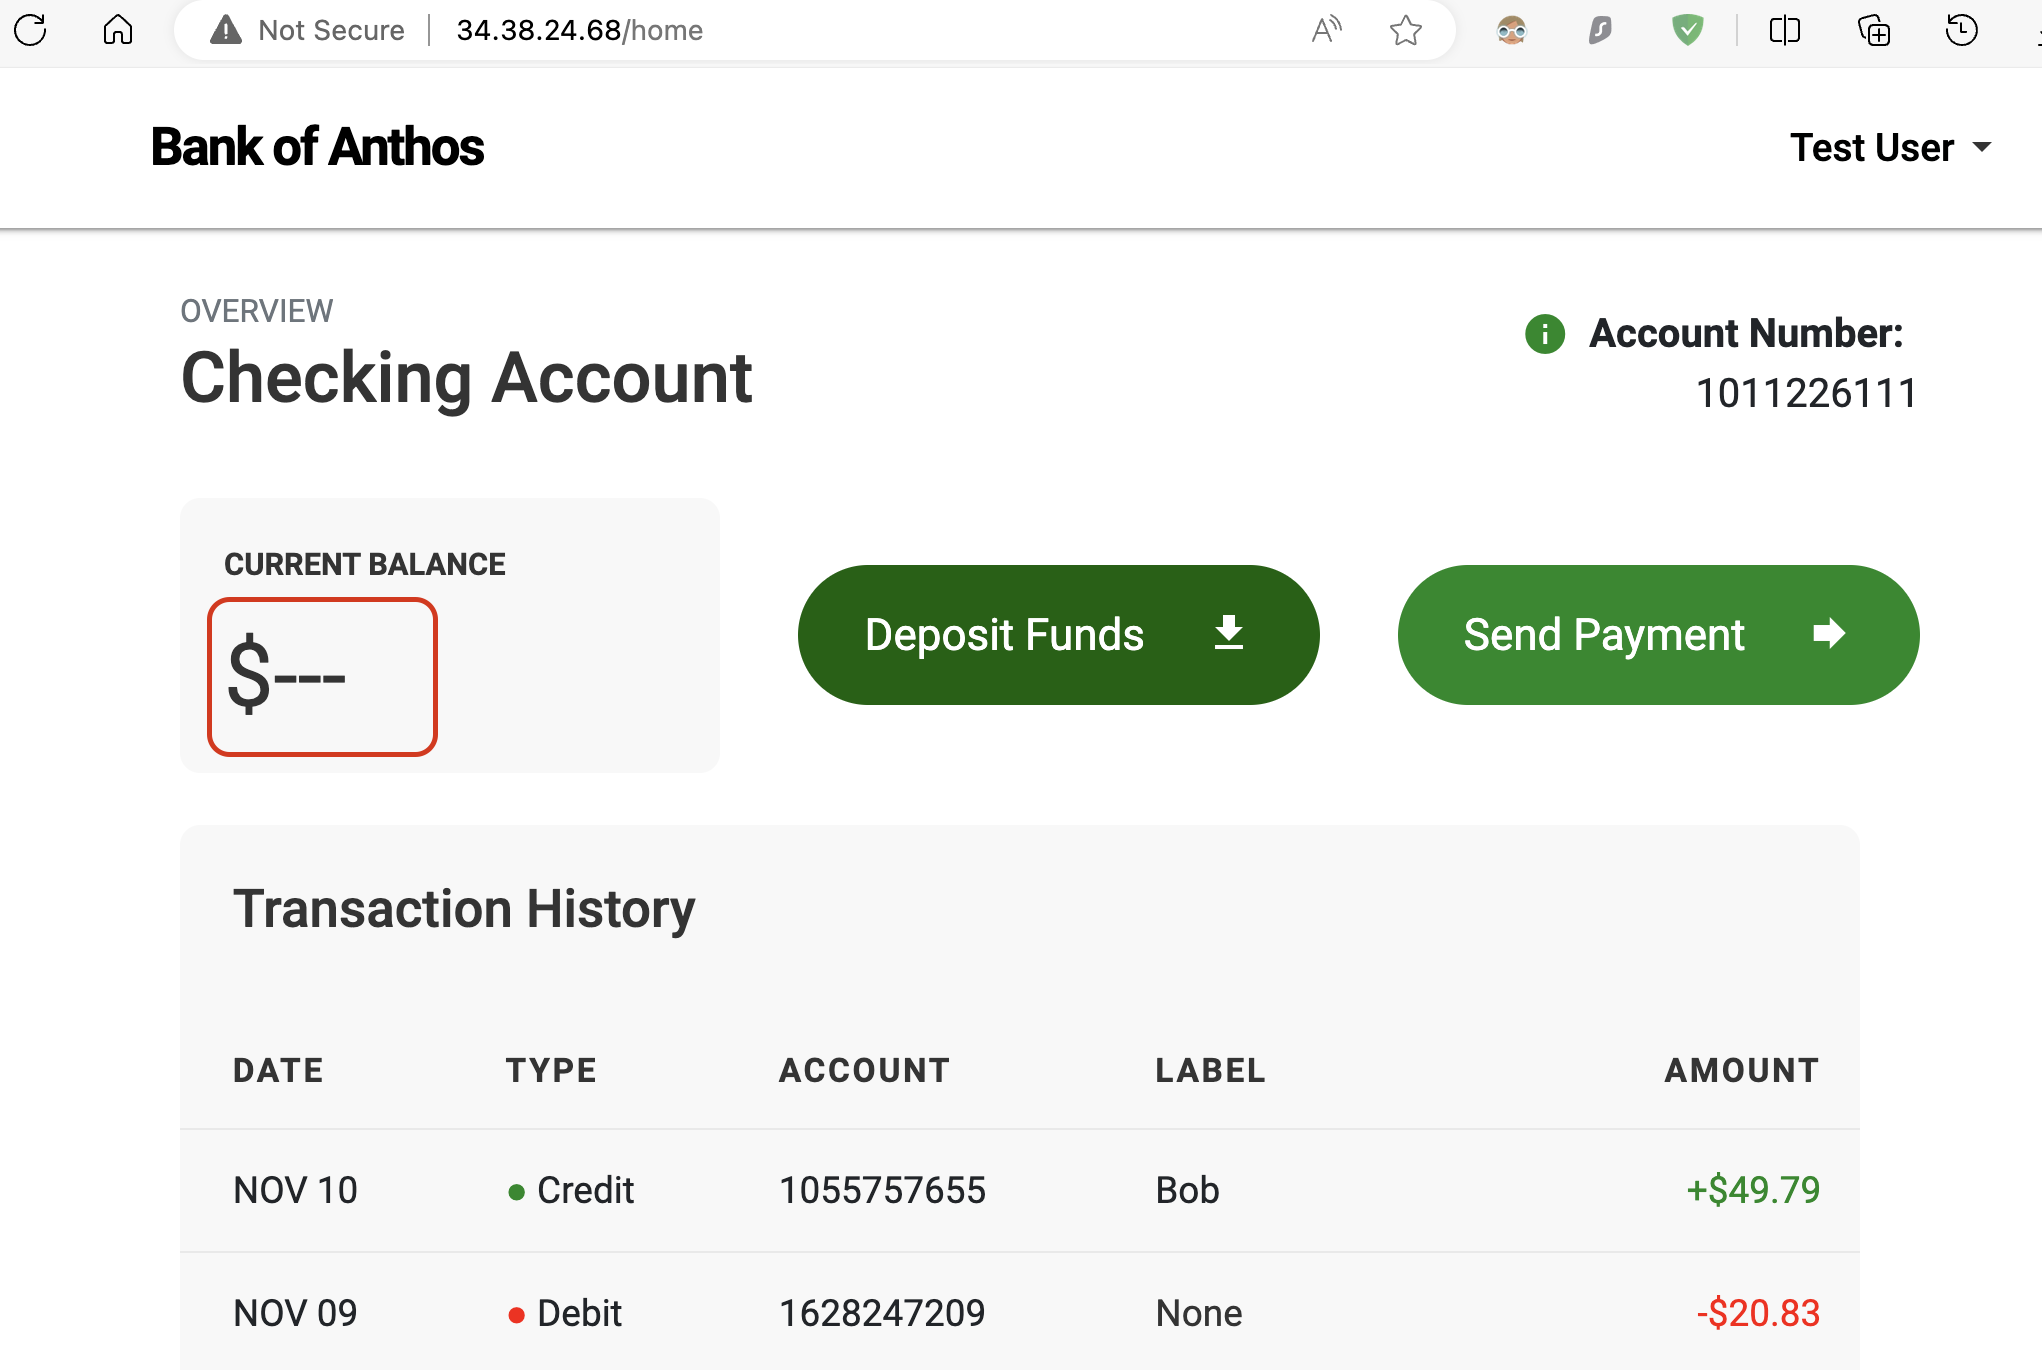
\includegraphics[width=1.0\linewidth]{resources/l7-policy-applied.png}
    \caption{Result of Waypoint L7 policy enforcement}
    \label{method:l7PolicyAppliedView}
\end{figure}


\subsection{Challenges Encountered}
\subsubsection{Ztunnel Blocks Service Start}
While setting up Istio with ambient mode, couple of microservices pods were stuck in Running state till the Ztunnel pod on the specific node was restarted. The configuration was:

\begin{itemize}
\item Istio with ambient profile installed on 3 nodes
\item 1 replica of all 8 microservices were deployed to a single node
\item Microservice deployment was done post Istio installation and namespace labelling
\end{itemize}

This scenario could not be reproducible all the time during the research, but this might be a point of interest for future investigations.

\subsubsection{Grafana Cloud Integration}
Grafana Cloud was chosen at first as a monitoring platform to retain research test data for a long period of time. After the Grafana cloud integration with the GKE instance was made, a few tests were done with Istio system data capture. This resulted in exceeding the free-tier metric limit of 10000 per month by 400\%. Later, the metric ingestion limit was controlled up to a certain limit by adding a filter in the Prometheus remote data export configuration; however, to avoid any unforeseen issues, switching to a Grafana local instance was preferred. Appendix \ref{appendix:grafana} mentions the details about setting up Grafana cloud integration.